\newpage
\section{Related Work}
\label{sec:RelatedWork}
In the following previous work in super-resolution, colorization and
task aware-downscaling are presented. At the end of each section the models
used for comparison and evaluation of the the underlying approach are further
explained in detail. Thereby the models were selected based on several criterias
performance compared to the state-of-the-art, the use as benchmark in related
papers and availability of (pretrained) models.

\subsection{Super-Resolution in Image Domain}
The problem of SR in the image domain is called \ac{SISR} and is shown in
\myfigref{fig:sisr_problem}. A lot of approaches have been
tried in order to cope with the \ac{SISR} problem. While early approaches such as
bicubic and Lanczos \cite{LFIOATD} tackle the problem using simple deterministic
filters which are computational cheap but produce blurry results and lack in
high frequency details, more recent approaches approach the problem using
example-based methods such as sparse encoding or deep learning methods.

\begin{figure}[!htbp]
	\centering
	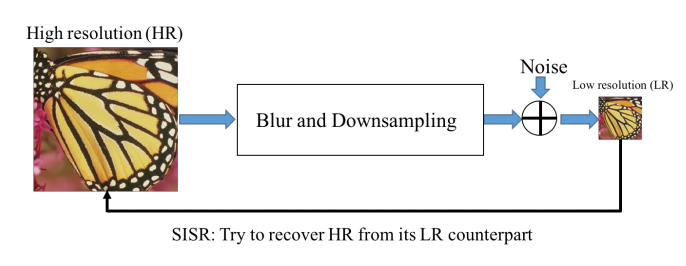
\includegraphics[width=14cm]{figures/sisr_problem}
	\caption{General SISR problem  according to \cite{DLFSISRABR}.}
  \label{fig:sisr_problem}
\end{figure}

Sparsity-based techniques assumes the \ac{LR} image to be transformable in another
domain (usually a dictionary of image atoms \cite{SARPFTTAISAIP}) and tries to
find correspondences between the \ac{LR} and \ac{HR} patches in the transformed space, as
implemented in \cite{IDASRBASDSAAR}. However, these techniques usually are
very computationally expensive. Among other learning based approaches such as
the use of random forests \cite{FAAIUWSRF}, in-place example regression models
\cite{FISRBOIPER} or adjusted anchored neighborhood regression \cite{AANRFFSR},
in terms of accuracy applying CNN based approaches have shown the largest success.
\footnote{An overview of various other deep learning based approaches for SISR
can be found in \cite{DLFSISRABR}.}
Dong et al. \cite{LADCNFISR} trained a shallow CNN end-to-end to build the HR
image based on a bicubicly upscaled LR image. This approach was improved by Kim
et al. \cite{AISRUVDCN} (VDSR) using a deeper network (20 layers) and cascading
small filters many times in a deep network structure to exploit contextual
information over large image regions in an efficient way. By advancing the
network model VDSR was further improved by Lim et al. \cite{EDRNFSISR} which
got the best results in the NTIRE2017 Super-Resolution Challenge \cite{NTIRE2017}.

\begin{figure}[!htbp]
	\centering
	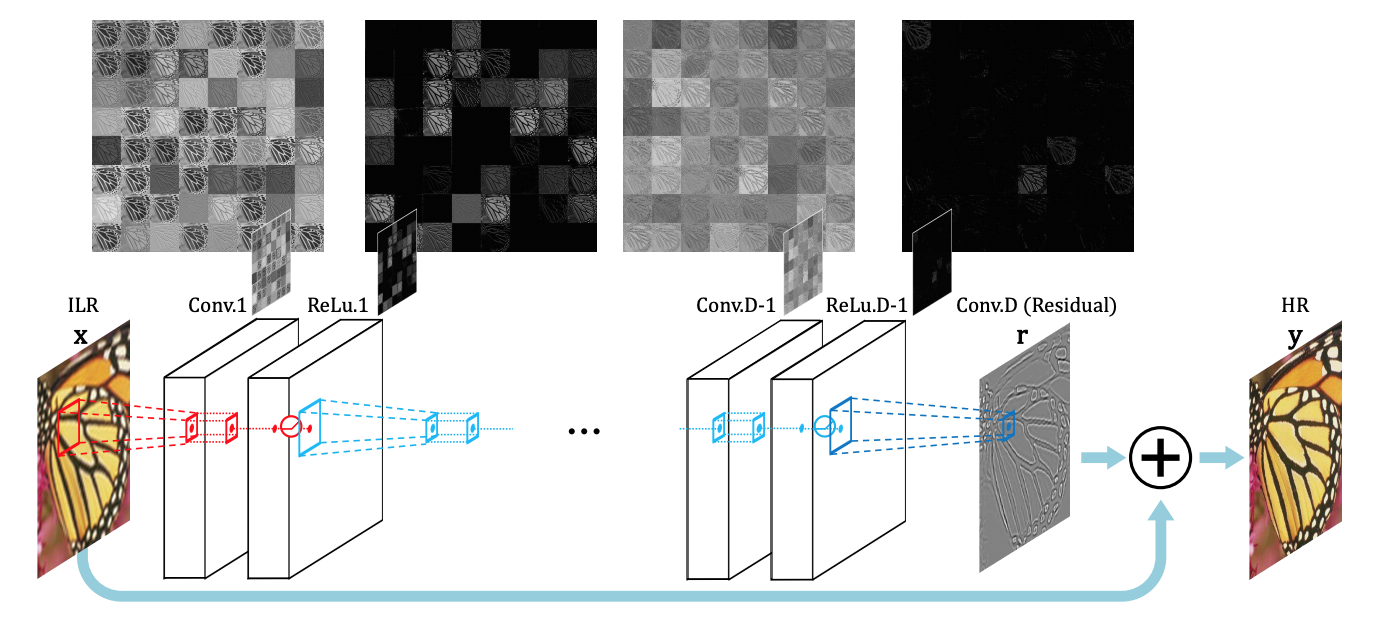
\includegraphics[width=14cm]{figures/vdsr}
	\caption{Overview of VDSR network design \cite{AISRUVDCN}.}
  \label{fig:vdsr}
\end{figure}

\subsection{Super-Resolution in Video Domain}
\ac{VSR} combines information from multiple adjacent LR frames
to take temporal information into account, leading to higher quality results.
Takeda et al. \cite{SRWESME} apply a 3D kernel regression on a patch of adjacent
\ac{LR} frames to implicitly encounter temporal information. Since purposed by
Caballero et al. \cite{RTVSRWSTNAMC} end-to-end approaches including motion
compensation such as the CNN framework from \cite{RTVSRWSTNAMC} have large success
in the VSR area. Liu et al. \cite{RVSRWLTD} added temporal addaptivity to the
framework to be able to aggregate the resulting \ac{HR} frame based on a weighted
sum of several estimates as well as a varying number of input LR frames. Sajjadi
et al. \cite{FRVSR} purposed a frame-recurrent architecture iteratively using
the previously inferred \ac{HR} frames for the subsequent prediction. Wang et al.
\cite{LFVSRTHROFE} (SOFVSR) implemented an end-to-end trainable approach to predict
both, the \ac{HR} frame as well as the HR optical flow. Therefore, first the HR
optical flow is inferred in a coarse-to-fine manner, then motion compensation is
performed according to the HR optical flows and finally, the compensated LR
inputs are fed to a super-resolution network to generate the HR frame estimate
(comp. \myfigref{fig:sofvsr}).

\begin{figure}[!htbp]
	\centering
	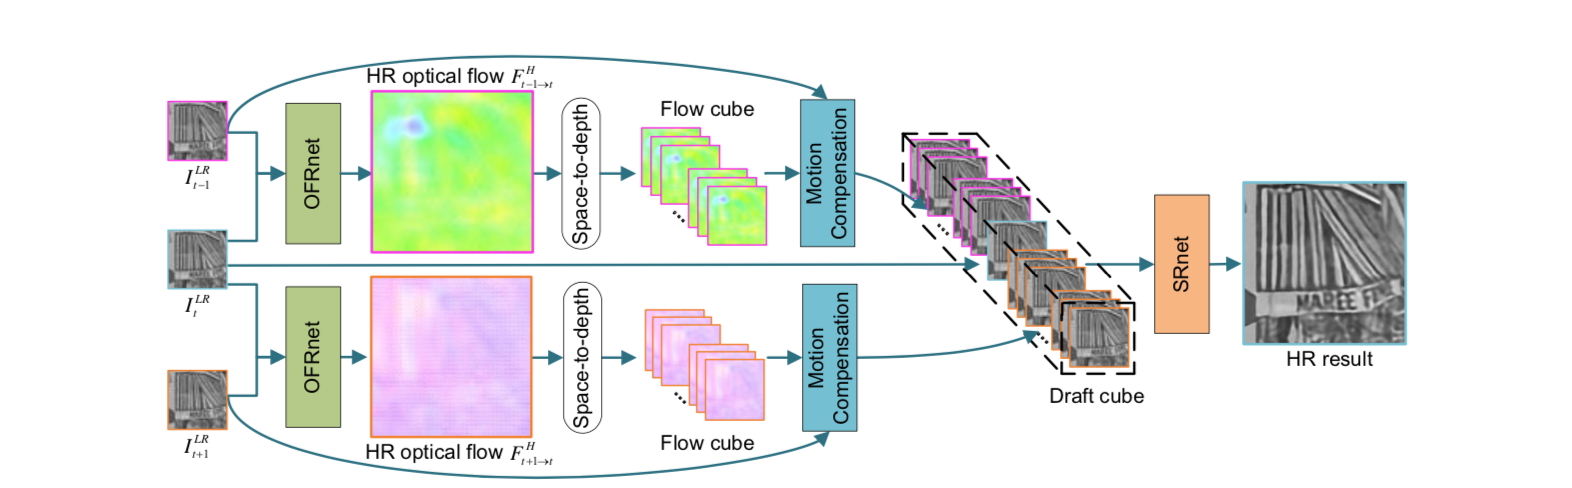
\includegraphics[width=14cm]{figures/sofvsr}
	\caption{Overview of SOFVSR pipeline \cite{LFVSRTHROFE}.}
  \label{fig:sofvsr}
\end{figure}

\subsection{Colorization}
Image colorization methods can be categorized in two categories: Non-parametric
approaches, such as \cite{ICUSI}, model the correspondence between the grayscale
and the colored image by finding analogeous regions in reference image(s),
while parameteric models learns this correspondence from large datasets,
transforming the colorization problem into a regression problem. Zhang et al.
\cite{CIC} (CIC) purpose posing colorization as a classification task and use
class-rebalancing at training time to increase the diversity of colors in the
result, using the CNN shown in \myfigref{fig:cic} and not requiring any
user-interaction.

\begin{figure}[!htbp]
	\centering
	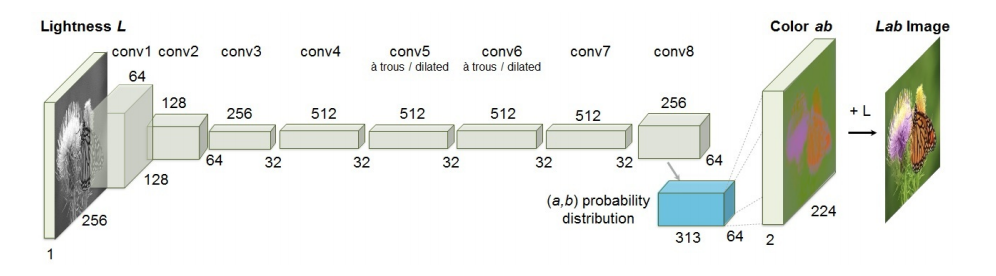
\includegraphics[width=14cm]{figures/cic}
	\caption{Overview of CIC network design \cite{CIC}.}
  \label{fig:cic}
\end{figure}

\subsection{Task-Aware-Downscaling}
Over all of the problems stated above most of the approaches merely take into
account one side of the process, e.g. by fixing the transformation HR to LR
to bicubic interpolation in order to large amount of training data and focusing
on estimating the inverse transformation. Kim et al. \cite{TAID} (TAID) purpose taking
into account the downscaling method in order to improve the upscaling performance,
by training an autoencoder in an end-to-end manner while the latent space
representation again is an image of same size as the LR image. The loss function
thereby contains both the difference between the decoded SHR and the original HR
image as well as the difference between the encoded SLR and the bicubic
interpolated LR image, such that the SLR image is a humanly understandable
representation. Next to SISR the approach is shown to be applicable for large
scale factor up to 128 as well as for colorization.


% Describe the other's work in the field, with the following purposes in mind:
%
% \begin{itemize}
%  \item \textit{Is the overview concise?} Give an overview of the most relevant work to the needed extent. Make sure the reader can understand your work without referring to other literature.
%  \item \textit{Does the compilation of work help to define the ``niche'' you are working in?} Another purpose of this section is to lay the groundwork for showing that you did significant work. The selection and presentation of the related work should enable you to name the implications, differences and similarities sufficiently in the ``discussion'' section.
% \end{itemize}
